\documentclass[conference]{IEEEtran}
\usepackage[T1]{fontenc}
\usepackage{amsmath,amssymb,graphicx,booktabs,array,microtype}
\usepackage[hidelinks]{hyperref}
\usepackage{url}
\newcommand{\framework}{CrowdScope}
\newcommand{\E}{\mathbb{E}}
\newcommand{\Prob}{\mathbb{P}}
\title{CrowdScope: A Modular Framework for Crowd-State Analysis and Uncertainty-Aware Resource Planning}
\author{\IEEEauthorblockN{Surya Maheswaran, Yashaswini Pawar, Sohan Kori, and Seema B. Hegde}
\IEEEauthorblockA{School of Computer Science and Engineering, RV University\\Bengaluru, Karnataka, India\\
\{suryam.btech23, yashaswinip.btech23, sohank.btech23, seemabhegde\}@rvu.edu.in}}
\begin{document}
\maketitle
\begin{abstract}
Crowd analysis requires more than an estimate of average walking speed: planners need spatial occupancy, movement conditions, population uncertainty, and an explicit connection between observations and decisions. This paper presents CrowdScope, a modular trajectory-to-decision framework combining geometry-aware density measurement, causal movement summaries, probabilistic composition estimation, and capacity-constrained resource allocation. Its interfaces separate observed crowd state, uncertain profile information, and application-specific service demand, allowing additional decision modules to be attached without treating demographic identity as a direct proxy for need. We evaluate the framework through three complementary evidence streams: recorded SiME trajectories, controlled planning experiments, and diagnostic pedestrian simulations. The recorded-data pipeline integrates 42 checkpoints from fourteen trials, while the fixed synthetic evaluation compares seven policies across fourteen conditions, sixty seed blocks, and 58,800 policy records. In the base condition, probabilistic allocation reduces mean unmet requests by 0.255 relative to a hard-posterior policy, with a paired 95\% bootstrap interval of $[-0.390,-0.127]$. However, it matches the stronger hard-observed policy in 599 of 600 allocations and provides no base-case advantage over that comparator. Small gains arise in selected secondary conditions. Simulation diagnostics expose unresolved clearance-time sensitivity. The framework therefore supports an auditable crowd-analysis workflow and a conditional assessment of information value, rather than universal claims of demographic recognition or evacuation improvement.
\end{abstract}
\begin{IEEEkeywords}
Conditional probability, crowd analysis, decision support, resource allocation, uncertainty quantification.
\end{IEEEkeywords}

\section{Introduction}
Crowds are spatially and behaviourally heterogeneous. The same number of occupants can create different conditions when they are distributed across several zones, concentrated at an entrance, or delayed behind a constrained passage. Recorded experiments show that mobility differences affect movement and interpersonal interactions in ways that a homogeneous average does not capture~\cite{sime,geoerg}. For a monitoring system, the immediate questions are therefore connected: where are people accumulating, how are they moving, what information about the population is uncertain, and which decisions would change if that uncertainty were resolved?

These questions are often addressed by separate tools. Trajectory processing produces positions and speeds; spatial analysis estimates density; perception systems classify individuals; and planning models allocate services or guide evacuation. Combining their outputs is not straightforward. A low speed can reflect congestion, waiting, geometry, or a movement limitation. A wheelchair label does not automatically establish a request for assistance. A precise class probability can improve a statistical score while leaving the optimal resource allocation unchanged. A useful framework must make these distinctions explicit.

We address this integration problem through \framework, an implemented modular framework for crowd-state analysis and decision support. It accepts time-stamped trajectories and walkable geometry, produces local occupancy and movement summaries, attaches probabilities from a declared information model, and passes the resulting state to an application-specific planner. The current decision module allocates a finite number of abstract support units to zones. An optional JuPedSim branch supports diagnostic what-if studies, while recording the numerical and behavioural limits of those studies.

The study investigates the \emph{decision value} of uncertainty through a fixed comparison with hard-posterior allocation and stronger hard-observed, population-only, and mean-demand controls. This distinguishes useful profile information from an incremental benefit of probability propagation.

The contributions are threefold. First, we implement a consistent trajectory-to-decision interface with geometry-aware measurement, past-only features, missingness flags, and explicit evidence labels. Second, we formulate and exactly solve a small conditional resource-allocation problem, linking uncertain profile membership to a separately specified demand mechanism. Third, we provide a reproducible comparison with negative controls, grouped uncertainty estimates, recorded-occupancy integration, and retained simulation failures. The mathematical components are established methods; the contribution lies in their transparent integration and the controlled analysis of when uncertain information changes a planning decision.

The architecture is reusable across applications that can supply compatible observations, zone definitions, and decision models. The present evaluation, however, covers recorded bottleneck occupancy and a static hypothetical service-allocation problem. Other uses, including routing, dynamic dispatch, and evacuation forecasting, require additional models and validation. We do not claim automatic wheelchair or child recognition, validated staffing recommendations, or a generally validated evacuation simulator.

\section{Literature Review and Related Work}
\subsection{Search strategy and evidence selection}
The focused review was updated on 4 November 2026, drawing on the preceding project's evidence register and targeted web searches of primary publisher, institutional, and author-repository sources. Actual query families included \emph{crowd trajectory disability wheelchair classification probabilistic resource allocation evacuation mobility uncertainty}; \emph{Bayesian crowd evacuation resource allocation uncertainty mobility impairment}; and quoted combinations of \emph{crowd}, \emph{composition}, \emph{uncertainty}, and \emph{planning}. No publication-year restriction was imposed. The cited literature spans foundational measurement and simulation methods through 2026.

We retained studies addressing heterogeneous movement, trajectory measurement, relevant recognition modalities, crowd-model uncertainty, or resource decisions. Unrelated infrastructure and surface-classification studies were excluded from the core comparison. Records were compared by DOI or repository identifier; access limits and unresolved checks were retained in the evidence ledger. We obtained no authenticated Scopus or Web of Science export and make no new PRISMA selection-count claim. The eighteen references below are a bibliography, not eighteen systematically screened empirical studies.

\subsection{Measurement, heterogeneity, and movement models}
SiME studies establish that visible mobility differences influence speed, spacing, and interactions at constrained passages~\cite{sime,geoerg}. Trajectory acquisition itself introduces measurement conventions: tracked head coordinates are not full-body footprints~\cite{boltes}. Density estimates also depend on spatial support; Voronoi measurement can reduce scatter compared with coarse fixed-region summaries~\cite{steffen}. \framework\ uses explicit zone area and observed membership, retaining the option of replacing its density estimator while keeping the downstream interface unchanged.

Established microscopic models provide different operational descriptions. Collision-free speed models adjust movement using available headway and interaction geometry~\cite{tordeux}; social-force models combine desired movement with interpersonal and obstacle interactions~\cite{helbing}. The Optimal Steps Model represents movement through continuous-space step selection~\cite{seitz}. JuPedSim supplies documented operational models and routing stages~\cite{jps}; the present diagnostic branch is pinned to version 1.4.2. Proximity or similar speed alone does not independently identify caregiving or assistance. Our earlier linkage experiments motivated retaining such relationships as an optional, separately validated input.

\subsection{Recognition and uncertainty-aware decisions}
Recognition-plus-prediction frameworks already exist. Lin \emph{et al.} combine LiDAR-derived size and movement features with pedestrian subclassification and arrival-time models~\cite{lin}. Their rule-derived labels illustrate why a movement rule cannot independently validate itself. V\'{a}squez \emph{et al.} detect mobility aids using depth imagery and probabilistic tracking~\cite{vasquez}; Woo \emph{et al.} provide smartphone/watch activity data for mobility-aid users~\cite{woo}. Neither modality establishes demographic recognition from the position-only trajectories used here. We therefore evaluate a declared noisy information channel instead of reporting a synthetic recogniser as a real detector.

Uncertainty in crowd models is also established. G\"odel \emph{et al.} compare point and Bayesian parameter calibration, showing that posterior structure can contain information omitted by a single fitted value~\cite{godel}. Von Schantz \emph{et al.} optimise rescue-guide configurations using probabilistic scenarios and mean/tail evacuation objectives~\cite{guides}. Moug \emph{et al.} formulate resource recruitment and routing under uncertain evacuation demand~\cite{moug}. Table~\ref{tab:literature} contrasts these tasks with ours. Our narrower question concerns the incremental effect of a profile-information representation on a fixed zone-allocation decision; it does not introduce Bayesian inference or stochastic planning.

\begin{table*}[t]
\caption{Selected methodological predecessors and the present evaluation scope}
\label{tab:literature}\centering\small
\begin{tabular}{>{\raggedright\arraybackslash}p{2.2cm}>{\raggedright\arraybackslash}p{2.8cm}>{\raggedright\arraybackslash}p{3.1cm}>{\raggedright\arraybackslash}p{3.2cm}>{\raggedright\arraybackslash}p{4.0cm}}
\toprule Study & Objective and method & Data or sample & Relevant finding & Boundary relative to this study\\\midrule
Geoerg et al.~\cite{sime,geoerg} & Analyse heterogeneous movement experimentally & SiME controlled passage trials & Composition changes movement/interactions & Supplied identity information does not validate our recogniser or service demand\\
Lin et al.~\cite{lin} & Subclassification and arrival prediction & LiDAR trajectories; rule-derived labels & Recognition and time estimation can be integrated & Appearance/size features and label construction differ from position-only inference\\
G\"odel et al.~\cite{godel} & Bayesian versus point calibration & Bottleneck model case studies & Posterior uncertainty reveals parameter structure & Parameter uncertainty differs from uncertain occupant metadata\\
von Schantz et al.~\cite{guides} & Guide planning; mean--CVaR optimisation & Simulated passenger terminal & Plans depend on uncertain crowd scenarios & Optimises evacuation dynamics rather than static service shortfall\\
Moug et al.~\cite{moug} & Stochastic recruitment and routing & Regional networks and demand scenarios & Uncertain demand changes resource decisions & Transport logistics includes temporal routing absent from our abstraction\\
Present study & Measure state; compare information-to-decision policies & 42 recorded checkpoints; fixed synthetic benchmark & Base decisions nearly invariant to probability versus hard observations & No independent recognition, real demand, or universal simulation validation\\\bottomrule
\end{tabular}
\end{table*}

The review supports a bounded research opportunity: an auditable comparison that distinguishes representation quality from decision changes, while keeping observed state, hypothetical composition, and assumed demand separate. It does not establish that no related integration exists. We position the work as an exploratory systems and benchmark contribution with explicit coverage limits.

\section{Research Problem, Objectives and Hypotheses}
Let a crowd observation at time $t$ comprise trajectories $\mathcal{X}_{\leq t}$ and walkable geometry $G$. The problem is to construct a state $S_t$ that supports both descriptive analysis and a resource decision $a_t$, while preserving uncertainty about information unavailable from trajectories. The objectives are to measure zone state consistently, estimate composition under a stated information model, allocate limited capacity, and evaluate whether retaining probabilities changes realised service shortfall.

Three research questions guide the study. RQ1 asks whether the measurement and decision modules can be connected to recorded trajectories without leaking future observations into state features. RQ2 asks whether probabilistic profile information improves allocation relative to hard labels and population information. RQ3 asks how the result changes under zone imbalance, resource limits, observation errors, and misspecified assumptions.

The primary endpoint is the paired difference in realised unmet requests, probabilistic minus hard posterior. The directional research hypothesis is $H_1:\E[\Delta]<0$, against $H_0:\E[\Delta]\geq0$, under the base synthetic mechanism. We report a paired bootstrap interval rather than an unqualified significance label. Comparisons with hard observed labels, population information, and mean-only planning remain essential controls. The primary comparator and its tie convention were retained even after development exposed its weakness; we do not replace it retrospectively with a favourable secondary condition.

The independent variable is the information representation supplied to a common planning objective. The dependent variable is realised unmet requests. Controlled quantities include initial roster, zone counts, budget, capacity, and paired random draws. Sensitivity factors include prevalence, observation error, demand rates, probability distortion, and zone imbalance. Repeated metadata/request replicas within a seed are dependent; the seed block is the independent unit for the synthetic comparison. In recorded data, repeated participants, geometry, partial visibility, and tracking quality constrain interpretation.

\section{Research Methodology}
\subsection{Framework architecture and interfaces}
We use a quantitative design-science approach: implement a modular artefact, verify its mathematical and data interfaces, and evaluate its behaviour through complementary evidence streams. Fig.~\ref{fig:architecture} summarises the workflow. A canonical trajectory record contains a run-local person identifier, time in seconds, and planar position in metres. The geometry interface supplies walkable polygons, obstacles, and analysis zones. A state record contains visible occupancy, density, speed/stopping summaries, observation coverage, and optional probabilities. Decision modules consume that record and an explicit application configuration.

\begin{figure*}[t]
\centering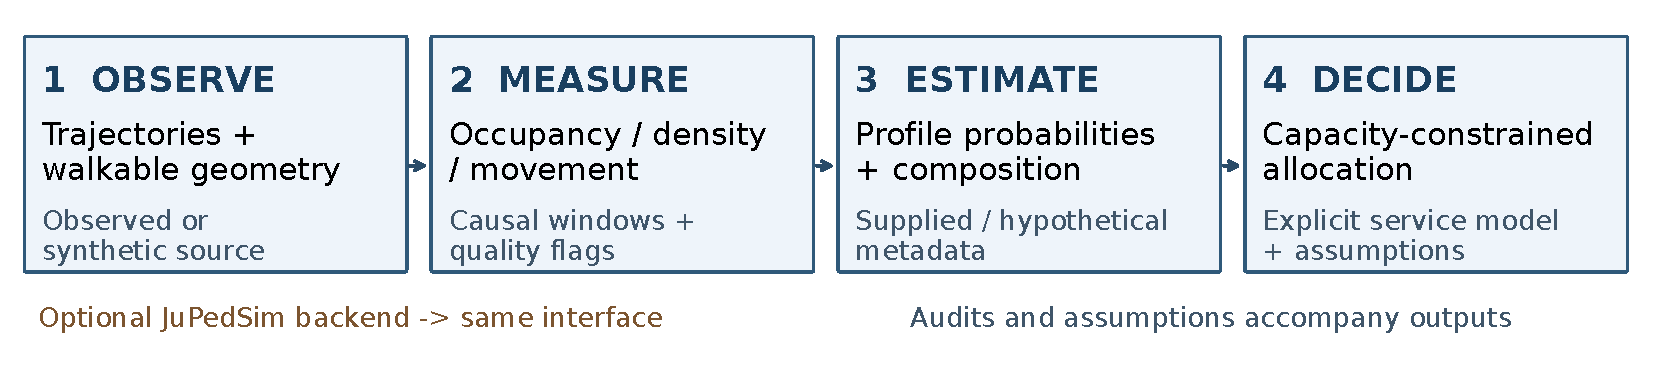
\includegraphics[width=.96\textwidth]{figures/architecture.pdf}
\caption{Implemented framework and evidence boundaries. Recorded trajectories validate occupancy integration; the information channel and service requests are controlled assumptions. Optional simulation is diagnostic. Additional applications require their own decision models and validation.}
\label{fig:architecture}
\end{figure*}

The interfaces separate acquisition, estimation, and application logic. A future recogniser can provide probabilities without changing the allocator, but needs independent calibration. Missing metadata retains the working prior with a flag; extra metadata cannot create occupants. Invalid numerical inputs, duplicate observations, overlapping zone interiors, and out-of-zone points produce explicit errors.

\subsection{Causal crowd-state measurement}
For zone $z$ with usable area $A_z$, visible occupancy and density are
\begin{equation}
N_z(t)=\sum_i\mathbf{1}\{p_i(t)\in z\},\qquad \rho_z(t)=N_z(t)/A_z.
\end{equation}
Polygon areas exclude obstacle holes. Shared boundaries belong to the lowest-numbered matching zone, and all currently observed occupants are assigned exactly once. Counts refer to the declared observation region; absent tracks are not automatically classified as building exits.

Movement features use only the past window $[t-h,t]$. Segment speed is Euclidean displacement divided by elapsed time, and a person's mean speed is total path length divided by valid observed duration. A gap larger than the source-specific maximum breaks continuity; only the contiguous suffix ending at the snapshot contributes. A lone observation has unknown speed rather than zero. Stopping uses a 0.1 m/s threshold, with both person stopped-time fraction and zone fraction of low-mean-speed occupants explicitly defined. We retain history coverage, complete-history flags, and missing-motion counts.

Snapshots use exact source timestamps without future interpolation or carry-forward. Crossing diagnostics count observed directional events rather than unique clearances. Early-stopped simulator checkpoints are unavailable, not empty crowds.

\subsection{Conditional composition model}
Let $C_i\in\{0,1\}$ denote a hypothetical mobility/service profile and $O_i$ a noisy supplied observation. In the controlled benchmark, $\Prob(C_i=1)=\pi$, with symmetric channel error $\eta$. Bayes' rule gives
\begin{align}
p_i^{(+)}&=\frac{\pi(1-\eta)}{\pi(1-\eta)+(1-\pi)\eta},\\
p_i^{(-)}&=\frac{\pi\eta}{\pi\eta+(1-\pi)(1-\eta)}.
\end{align}
This is an analytical information model, not a trained trajectory classifier. In a deployment model, $\Prob(C_i\mid X_i,E_i)$ would require independently supported labels and context $E_i$, including congestion and geometry. The current implementation does not infer disability, age, or assistance need from speed.

Expected zone composition is
\begin{equation}
\E[N_{z,1}\mid O]=\sum_{i\in z}p_i.
\end{equation}
Under the working independence assumption, the count distribution is Poisson-binomial. Its probabilities are computed recursively by convolving each Bernoulli membership, producing count intervals and variance $\sum_i p_i(1-p_i)$. Correlated errors and crowd-selection effects can invalidate that approximation. In particular, an initial population prior is not automatically calibrated among occupants remaining after selective exits. The fixed-roster benchmark avoids claiming that such survivor calibration has been established.

Probability scoring and allocation are distinct evaluations. We report the Brier score, the mean squared difference between probability and binary truth~\cite{brier}, alongside decision losses. A good probability score alone cannot establish useful resource recommendations.

\subsection{Application module: finite-capacity allocation}
Profile membership and demand are separate variables. Let $R_i$ indicate a request for the specified service, with scenario rates $r_0$ and $r_1$. The working request probability is
\begin{equation}
q_i=\Prob(R_i=1\mid O_i)=r_0+(r_1-r_0)p_i.
\end{equation}
The rates are assumed, not estimated from actual requests. A wheelchair user is not automatically assigned a request. For zone demand $D_z=\sum_{i\in z}R_i$, integer allocations $a_z$, budget $B$, and per-unit capacity $k$, the planner solves
\begin{align}
a^*&=\arg\min_{a\in\mathcal{A}}\E\!\left[\sum_z(D_z-ka_z)_+\mid O\right],\\
\mathcal{A}&=\{a\in\mathbb{Z}_{\geq0}^{Z}:\sum_z a_z=B\}.
\end{align}
Here $(x)_+=\max(0,x)$. Zone demand uses the analogous Poisson-binomial recursion over request probabilities. Four zones and six units have $\binom{9}{3}=84$ allocations, allowing exact enumeration rather than a heuristic. Cost ties within $10^{-12}$ use the lexicographically first allocation. Units are interchangeable and assumed prepositionable without travel delay; the model represents one planning epoch, not dynamic dispatch or clinical staffing.

The mean-demand ablation minimises $\sum_z(\E[D_z]-ka_z)_+$ instead. Nonlinearity means this can differ from expected shortfall, although the policies can also make identical decisions. Perfect-demand allocation is computed only as a non-deployable hindsight lower bound. Realised requests never enter any deployable planner.

\subsection{Evidence streams and evaluation design}
The recorded-data branch reads fourteen archived SiME trials~\cite{dataset}, with 1,151 person-trial tracks. Seven documented wheelchair participants repeat across the eight relevant runs; 56 such observations are not 56 independent people. Most tracks lack verified persistent identities. We therefore do not create an unseen-person recognition claim or treat unregistered tracks as confirmed negatives.

For integration, the observable area is the official walkable geometry intersected with $x\in[-6,2.4]$ and $y\in[-1.65,1.65]$ m. Four zones split $x$ at $-6,-3,-1,0,2.4$. Checkpoints are 10, 20, and 30 s, with two-second histories at 25 Hz. Service-profile observations are deliberately artificial and stable per trial-local track across checkpoints. This demonstrates interface composition without assigning actual disabilities or assistance needs. Trial 1307 retains a metadata/track count discrepancy; trial 507 lacks an observed downstream crossing for one track. Neither issue is hidden by converting observation loss into an exit.

The synthetic planning branch uses eighty occupants in four fixed zones, initially twenty per zone. Base settings are $\pi=0.2$, $\eta=0.2$, $r_0=0.1$, $r_1=0.4$, $B=6$, and $k=2$. These are experimental choices, not population estimates or safety standards. Class membership is sampled per seed block, then held fixed across ten independent observation/request replicas. Separate deterministic streams generate classes, channel errors, and requests, with common uniforms supporting paired sensitivity comparisons.

Seven policies are retained: population prior, hard observed ($p_i=O_i$), hard posterior ($p_i=\mathbf{1}\{p_i>0.5\}$), probabilistic, mean-demand, known class, and perfect demand. The known-class policy still does not know realised requests. At the base settings, a positive observation has posterior 0.5, so the frozen hard-posterior tie rule labels every observation negative. We retain this comparator for protocol integrity and explicitly test stronger alternatives.

Fourteen predeclared conditions cover unequal zone counts $[40,24,12,4]$, budgets three/nine, perfect/uninformative channels, low/high true prevalence, underestimated channel error, probability temperatures 0.5/2, equal demand, demand misspecification, and higher demand contrast. Exact values are supplied with the code. Development and validation used distinct seed ranges. The final comparison uses sixty reserved seed blocks, ten replicas per condition, and all fourteen conditions: 8,400 replicas and 58,800 policy records.

We average replicas within seed before statistical analysis. The primary paired mean difference uses a percentile block-bootstrap interval with 10,000 resamples and seed 9041, following the resampling principle~\cite{efron}. Keeping related observations together addresses the dependence concerns underlying structured validation~\cite{roberts}. Secondary intervals are descriptive and not multiplicity-adjusted. The number of blocks is a fixed computational budget, not a power-derived sample size. No model selection follows final-outcome inspection.

\subsection{Verification, simulation, and research ethics}
Forty-two automated tests cover trajectory units, known speeds/densities, boundary assignments, gaps, future invariance, probability identities, polygon holes, exact planning, and evaluation guards. Independent saved-output audits check conservation, budgets, realised losses, grouping, and negative controls. Experiment configurations and source hashes are recorded before execution. The release record preserves a pre-execution path-key correction; no model or analysis choice changed.

JuPedSim~\cite{jps} is an optional diagnostic backend. Small walker, pair, doorway, queue, and turn fixtures pass spatial checks, but larger crowds expose jams and timestep sensitivity. We retain them rather than declaring a universal simulator. A separate matched reference replay uses actual SiME geometry and observed future inlet events; it is not an evacuation forecast. Circle overlap and wall-penetration thresholds are 0.001 and 0.005 m. Source-matched head-centre crossings remain distinct from full-circle exits in generic fixtures.

No participants were recruited for this study. Raw and derived person-level SiME trajectories remain local pending confirmation of redistribution terms; synthetic benchmark inputs and aggregate results support reproducibility. No new ethics approval is claimed, and no deployment or demographic diagnosis is performed.

\section{Results}
\subsection{Recorded crowd-state integration}
All 42 SiME checkpoints integrate without in-window geometry mismatch. Zone counts sum to the visible in-region roster, density uses obstacle-aware usable area, probability distributions sum to one, and allocations satisfy the budget. The 1307 metadata discrepancy remains flagged. These results verify processing and evidence separation, not accuracy of hypothetical profile labels or the effectiveness of staffing recommendations. Repeated participants and checkpoints preclude treating the observations as 42 independent population samples.

\subsection{Primary policy comparison}
Table~\ref{tab:primary} reports base mean losses. Probabilistic planning reduces unmet requests from 3.431667 to 3.176667 relative to hard posterior, a difference of $-0.255$ requests per scenario with paired 95\% interval $[-0.390,-0.126667]$. Thirty-five seed blocks improve, seven tie, and eighteen worsen. Population-only and hard-posterior policies share the same base mean; the threshold weakness described above is therefore material to the interpretation.

\begin{table}[t]\centering
\caption{Base synthetic evaluation: unmet requests per scenario}
\label{tab:primary}\small
\begin{tabular}{lrr}\toprule Policy & Mean & SD of block means\\\midrule
Population prior & 3.4317 & 1.1043\\
Hard posterior & 3.4317 & 1.1043\\
Hard observed & 3.1750 & 0.9745\\
Probabilistic & 3.1767 & 0.9766\\
Mean demand & 3.1767 & 0.9766\\
Known class & 2.9617 & 1.0088\\
Perfect demand (hindsight) & 1.9633 & 0.9620\\\bottomrule
\end{tabular}
\end{table}

Against hard observed, the difference is instead $+0.001667$, interval $[0,0.005]$. Their allocations agree in 599 of 600 replicas; 59 block effects tie and one favours hard observed. The probabilistic and mean-demand allocations agree in all 600 base replicas. Consequently, the primary gain does not establish incremental value over hard observed or a full-distribution advantage over mean-only planning in this setting. We did not prespecify an equivalence margin and do not claim formal equivalence.

Known-class information reduces the base mean to 2.961667, while the non-deployable perfect-demand reference gives 1.963333. Their gap reflects request uncertainty and capacity constraints, not solely recognition error.

\subsection{Sensitivity and decision agreement}
Fig.~\ref{fig:effects} summarises secondary effects against hard observed. Unequal zones yield a mean difference of $-0.065$, descriptive interval $[-0.100,-0.030]$, with 79\% allocation agreement. Higher demand contrast yields $-0.045$, interval $[-0.073333,-0.016667]$, and approximately 90.8\% agreement. The nine-unit condition gives a smaller difference of $-0.006667$, interval $[-0.015,0]$. These are conditional descriptive results, not replacements for the base comparison or multiplicity-adjusted confirmatory claims.

\begin{figure}[t]\centering
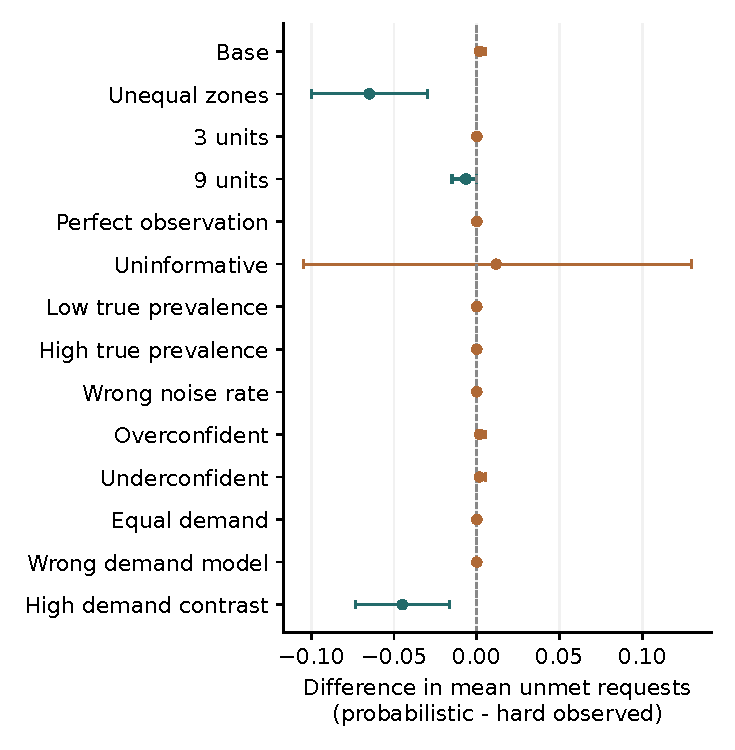
\includegraphics[width=\columnwidth]{figures/effects.pdf}
\caption{Probabilistic minus hard-observed unmet requests across all fourteen conditions. Negative values favour probabilities. Intervals are paired seed-block percentile intervals; secondary comparisons are descriptive.}
\label{fig:effects}
\end{figure}

Uninformative observations correctly return the prior. The mean difference from hard observed is $+0.011667$, interval $[-0.105,0.130]$, showing that random fluctuations in noisy-label decisions cannot be interpreted as useful information. Under perfect observations, probabilistic and known-class allocations coincide. When modelled request rates are equal across classes, all full-distribution information variants choose the same allocation. Mean-only planning can still differ because it changes the objective rather than the information.

The base Brier score is approximately 0.117746, close to the analytical matched-channel value 0.117647. Yet allocation agreement with hard observed is nearly complete. Prior, noise, and temperature changes alter probability quality without necessarily changing decisions. Development patterns of harm under low prevalence do not uniformly reproduce in the final sample, reinforcing the need to retain independent outcomes instead of presenting pilot trends as general laws.

\subsection{Simulation diagnostics}
The generic eighty-person room and corridor initially fail to clear within 120 s. Routing ablations do not resolve the jam at matched settings. Small position perturbations and a wider entrance permit completion in some runs, but finer timesteps alter completion or clearance beyond the recorded tolerance. An AVM candidate fails wall checks. These failures remain available with successful small fixtures.

Matched reference replays provide more bounded evidence. At timestep 0.0025 s, trials 1501 and 1507 complete with individual head-crossing MAE 4.237 and 2.720 s, compared with same-arrivals free-flight MAE 16.195 and 10.656 s. At 0.00125 s, both complete with MAE 5.814 and 2.495 s. First-to-last simulated crossing spans change by 1.555 and 1.539 s between these finest settings, exceeding the 1\% criterion. Thus interactions improve these conditional replays relative to free flight, but stable general clearance prediction is not established. All reference trials were previously used in development.

\section{Discussion}
\subsection{From accurate state to useful decisions}
The principal finding is a distinction between state uncertainty and decision value. CrowdScope can retain uncertain composition and compute an exact expected-loss allocation, but that does not guarantee a different or better action than a hard-label policy. In the balanced base problem, most changes in probability representation leave the allocation unchanged. The unequal-zone and higher-contrast conditions show that different capacity/demand configurations can make those distinctions consequential, although the observed gains remain small.

A crowd-analysis framework should expose whether uncertain composition changes the action, how much loss is at stake, and which demand assumptions drive the recommendation. Probability estimates can communicate uncertainty even when the allocation matches a simpler baseline.

The controls prevent an overly broad interpretation: the base improvement reflects usable information relative to an uninformative policy, while neither probability propagation nor the nonlinear objective consistently changes the decision. Loss differences and decision disagreement should therefore be reported together.

\subsection{Extensibility and application boundaries}
The framework's reusable object is the crowd-state interface, not a universal policy. Occupancy management can consume counts, usable area, speed, and observation coverage. Accessibility-oriented monitoring can consume validated supplied metadata or a separately calibrated recognition model. A routing module could consume zone congestion and travel-time estimates; a dynamic service module would additionally need travel, queueing, and service-duration models. Evacuation forecasting would require a validated operational model, arrival/route assumptions, and a precisely defined safety endpoint.


\subsection{Threats to validity}
The most important construct limitation is that hypothetical profile membership is not observed disability or actual assistance need. Movement alone may not identify semantic classes because congestion and geometry can produce similar patterns. The current evidence therefore cannot validate automatic identification of children, older adults, or wheelchair users. The missing demand annotations additionally make resource outcomes conditional on chosen rates rather than empirical service success.

Internal validity is constrained by the analytical channel and independent-request mechanism. Shared-context errors, correlated requests, spatially clustered needs, observation loss, and dynamic travel costs could change the result. Exact optimisation under a known working distribution is not evidence that the distribution is correct. The benchmark deliberately tests misspecification but does not cover every deployment shift.

External validity is limited by one dataset family, repeated SiME participants, restricted observation regions, fixed synthetic rosters, and a computationally chosen sample size. The review is focused rather than exhaustive, and the framework assembles established methods. We do not assert a verified first implementation. The generic simulator failures prevent operational clearance claims and illustrate why a complete-looking application cannot substitute for movement validation.

Secondary cells share seeds and use unadjusted intervals; development informed the exploratory design. All outcomes are retained.

\section{Conclusion and Future Work}
CrowdScope connects trajectory ingestion, geometry-aware crowd measurement, uncertain composition, and explicit resource decisions within one reproducible framework. Recorded-data integration succeeds at 42 checkpoints, while the controlled evaluation shows that probability quality and planning benefit are not interchangeable. The base gain over hard posterior does not extend to the stronger hard-observed comparator; small secondary gains depend on occupancy and demand structure. Negative controls and retained simulation failures define the boundaries of those findings.

The next priorities are independently annotated motion data, context-aware probability calibration, and an empirically grounded service-demand model. Dynamic dispatch should incorporate travel/service times and reassignment costs; correlated demand should replace independence where supported. A future motion recogniser must be evaluated on unseen people with suitable negatives and abstention, without labelling slow movement as disability. Simulation work should resolve geometry/contact and timestep sensitivity before supporting clearance forecasts. These extensions would broaden the framework through validated modules rather than an unsupported claim of universal applicability.

\smallskip\noindent\textit{Declarations and availability.}
No external funding was received. No new participants were recruited. Synthetic benchmark configurations, code, aggregate results, audit scripts, and a labelled demonstration are provided in the private project repository: \url{https://github.com/surya070/crowd-clearance-forecasting}. Access requires repository permission. Raw and derived participant-level trajectories are excluded from the repository update pending confirmation of redistribution terms. The demonstration distinguishes synthetic observations and assumed requests from real-data validation. Author declarations and venue-specific requirements should be confirmed before formal submission.

\begin{thebibliography}{18}
\bibitem{sime} P. Geoerg, J. Schumann, M. Boltes, and M. Kinateder, ``How people with disabilities influence crowd dynamics of pedestrian movement through bottlenecks,'' \emph{Scientific Reports}, vol. 12, art. 14273, 2022, doi: 10.1038/s41598-022-18142-7.
\bibitem{geoerg} P. Geoerg, J. Schumann, S. Holl, and M. Boltes, ``The influence of individual impairments in crowd dynamics,'' \emph{Fire and Materials}, vol. 45, no. 4, pp. 529--542, 2021, doi: 10.1002/fam.2789.
\bibitem{boltes} M. Boltes and A. Seyfried, ``Collecting pedestrian trajectories,'' \emph{Neurocomputing}, vol. 100, pp. 127--133, 2013, doi: 10.1016/j.neucom.2012.01.036.
\bibitem{steffen} B. Steffen and A. Seyfried, ``Methods for measuring pedestrian density, flow, speed and direction with minimal scatter,'' \emph{Physica A}, vol. 389, pp. 1902--1910, 2010, doi: 10.1016/j.physa.2009.12.015.
\bibitem{tordeux} A. Tordeux, M. Chraibi, and A. Seyfried, ``Collision-free speed model for pedestrian dynamics,'' in \emph{Traffic and Granular Flow '15}, Springer, 2016, pp. 225--232, doi: 10.1007/978-3-319-33482-0\_29.
\bibitem{helbing} D. Helbing and P. Moln\'{a}r, ``Social force model for pedestrian dynamics,'' \emph{Physical Review E}, vol. 51, pp. 4282--4286, 1995, doi: 10.1103/PhysRevE.51.4282.
\bibitem{seitz} M. J. Seitz and G. K\"oster, ``Natural discretization of pedestrian movement in continuous space,'' \emph{Physical Review E}, vol. 86, art. 046108, 2012, doi: 10.1103/PhysRevE.86.046108.
\bibitem{jps} JuPedSim developers, ``JuPedSim: pedestrian models and API documentation,'' software v1.4.2 used in this study. [Online]. Available: \url{https://www.jupedsim.org/}. Accessed: Nov. 4, 2026.
\bibitem{lin} T. Lin, Z. Jin, S. Choi, and H. Yeo, ``A framework for pedestrian sub-classification and arrival time prediction at signalized intersection using preprocessed Lidar data,'' arXiv:2201.05877, 2022.
\bibitem{vasquez} A. V\'{a}squez, M. Kollmitz, A. Eitel, and W. Burgard, ``Deep detection of people and their mobility aids for a hospital robot,'' arXiv:1708.00674, 2017.
\bibitem{woo} Y. Woo et al., ``Human activity recognition dataset for pedestrians with mobility disabilities,'' \emph{Scientific Data}, vol. 13, art. 211, 2026, doi: 10.1038/s41597-025-06527-y.
\bibitem{godel} M. G\"odel, N. Bode, G. K\"oster, and H.-J. Bungartz, ``Bayesian inference methods to calibrate crowd dynamics models for safety applications,'' \emph{Safety Science}, vol. 147, art. 105586, 2022, doi: 10.1016/j.ssci.2021.105586.
\bibitem{guides} A. von Schantz, H. Ehtamo, and S. Hostikka, ``Minimization of mean-CVaR evacuation time of a crowd using rescue guides: A scenario-based approach,'' arXiv:2010.03922v2, 2021.
\bibitem{moug} K. Moug, H. Jia, and S. Shen, ``A shared mobility based framework for evacuation planning and operations under forecast uncertainty,'' author preprint, 2020. [Online]. Available: \url{https://optimization-online.org/wp-content/uploads/2020/08/7963.pdf}
\bibitem{brier} G. W. Brier, ``Verification of forecasts expressed in terms of probability,'' \emph{Monthly Weather Review}, vol. 78, no. 1, pp. 1--3, 1950.
\bibitem{dataset} P. Geoerg et al., ``Influence of individual characteristics,'' \emph{Pedestrian Dynamics Data Archive}, dataset, doi: 10.34735/ped.2017.1.
\bibitem{efron} B. Efron, ``Bootstrap methods: Another look at the jackknife,'' \emph{The Annals of Statistics}, vol. 7, no. 1, pp. 1--26, 1979, doi: 10.1214/aos/1176344552.
\bibitem{roberts} D. R. Roberts et al., ``Cross-validation strategies for data with temporal, spatial, hierarchical, or phylogenetic structure,'' \emph{Ecography}, vol. 40, pp. 913--929, 2017, doi: 10.1111/ecog.02881.
\end{thebibliography}
\end{document}
